\section{Duality theory}

These notes are based on earlier lecture notes by Benjamin Recht and Ashia
Wilson.

\subsection{Optimality conditions for equality constrained optimization}

Recall that $x_\star$ minimizes a smooth, convex function $f$ over a closed convex set $\Omega$ if and only if 
 \begin{equation}\label{eq:opt-cond}
  \langle \nabla f(x_\star), x - x_\star \rangle \geq 0 \;\;\;\; \forall x \in \Omega\,.
 \end{equation}

Let's specialize this to the special case where $\Omega$ is an affine set.  Let $A$ be an $n\times d$ matrix with rank $n$ such that $\Omega =\{x~:~Ax=b\}$ for some $b\in \R^n$.  Note that we can always assume that $\operatorname{rank}(A) = n$ or else we would have redundant constraints. We could also parameterize $\Omega$ as  $\Omega = \{x_0 + v : Av= 0\}$ for any $x_0\in \Omega$.  Then using~\eqref{eq:opt-cond}, we have
  \begin{equation*} 
  \langle \nabla f(x_\star), x - x_\star \rangle \geq 0  ~~\forall x \in \Omega~~~\mbox{if and only if}~~~
    \langle \nabla f(x_\star), u \rangle \geq 0 ~~\forall u \in \operatorname{ker}(A)\,.
    \end{equation*}
But since $\operatorname{ker}{A}$ is a subspace, this can hold if and only if  $\langle \nabla f(x_\star), u \rangle = 0$ for all $u \in \operatorname{ker}(A)$.  In particular, this means, $\nabla f(x_\star)$ must lie in $\operatorname{ker}(A)^\perp$.  Since we have that $\R^d = \operatorname{ker}(A) \oplus \operatorname{Im}(A^T)$, this means that $\nabla f(x_\star) = A^T \lambda$ for some $\lambda \in \R^n$.

To summarize, this means that $x_\star$ is optimal for $f$ over $\Omega$ if and only if there $\exists \lambda_\star \in \R^m$ such that 
$$ \begin{cases}
   \nabla f(x_\star) + A^T \lambda_\star  = 0\\
  Ax_\star = b 
  \end{cases}$$
These optimality conditions are known as the \emph{Karush-Kuhn-Tucker Conditions} or \emph{KKT Conditions}.


As an example, consider the equality constrained quadratic optimization problem
\begin{equation*} 
  \begin{array}{ll} 
  \text{minimize} &\frac{1}{2} x^TQx + c^T x\\
  \text{subject to} &Ax = b 
  \end{array}
\end{equation*}
The KKT conditions can be expressed in matrix form
 $$\left[\begin{array}{cc} 
  Q &A^T\\
  A & 0 \end{array} \right]
    \left[\begin{array}{c} 
x\\
\lambda\end{array} \right] =  
\left[\begin{array}{c} 
c\\
b\end{array} \right] \,.$$


\subsection{Nonlinear constraints}

Let $\Omega$ be a closed convex set.  Let's define the \emph{tangent cone} of $\Omega$ at $x$ as 
\[
\mathcal{T}_{\Omega}(x) = \operatorname{cone} \{z - x : z \in \Omega\}
\]
The tangent cone is the set of all directions that can move from $x$ and remain in $\Omega$.  We can also define the \emph{normal cone} of $\Omega$ at $x$ to be the set
\[
	\mathcal{N}_{\Omega}(x) = \mathcal{T}_{\Omega}(x)^\circ = \left\{ u~:~ \langle u,v \rangle \leq 0,~~\forall v\in \mathcal{T}_{\Omega}(x) \right\} \,
\]

% \begin{figure}[h]
% \hspace{3cm}
% \includegraphics[width = 10cm]{normal_tangent_cone.pdf}
% \hspace{1cm}
% \includegraphics[width = 10cm]{normal_tangent2.pdf}
% \hspace{3cm}
% \end{figure}


\begin{figure}[h!]
    % \centering
    \vspace{-3cm}
    \hspace{-5cm}
    \begin{minipage}{0.45\textwidth}
        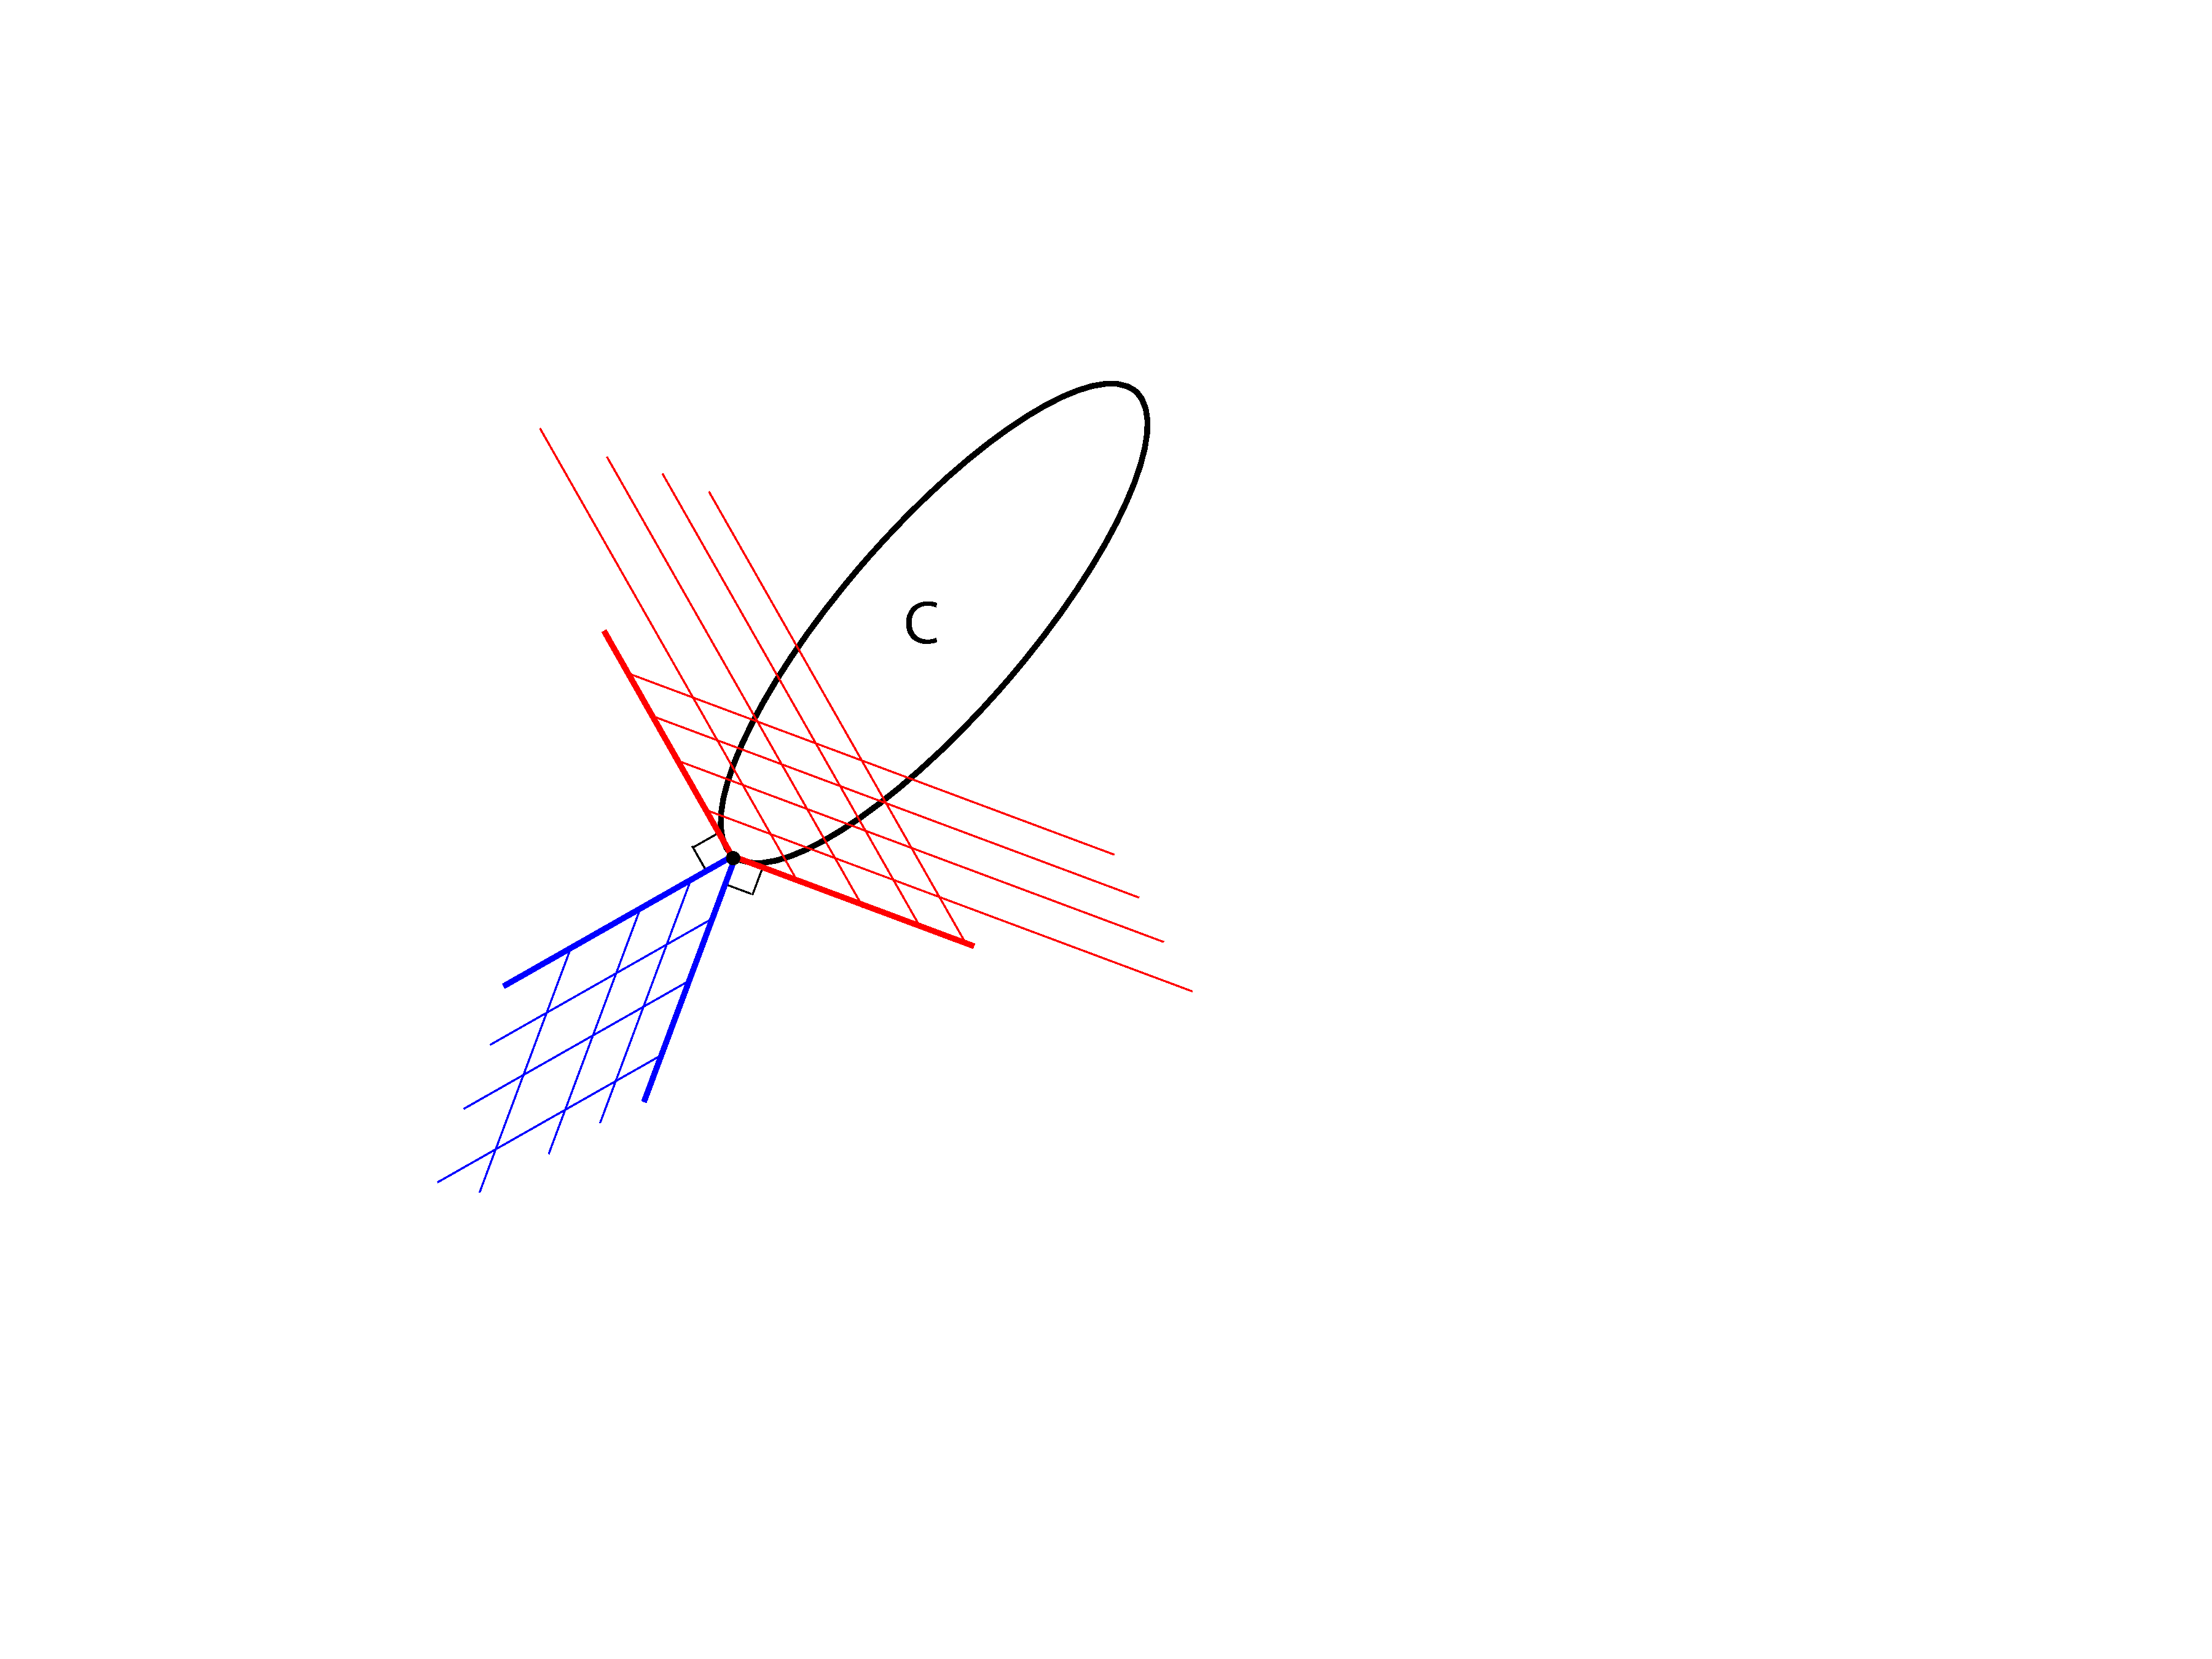
\includegraphics[width=3\textwidth]{figures/lecture13-normal_tangent_cone.pdf} % first figure itself
        % \caption{first figure}
    \end{minipage}\hfill
    \begin{minipage}{0.45\textwidth}
        % \centering
        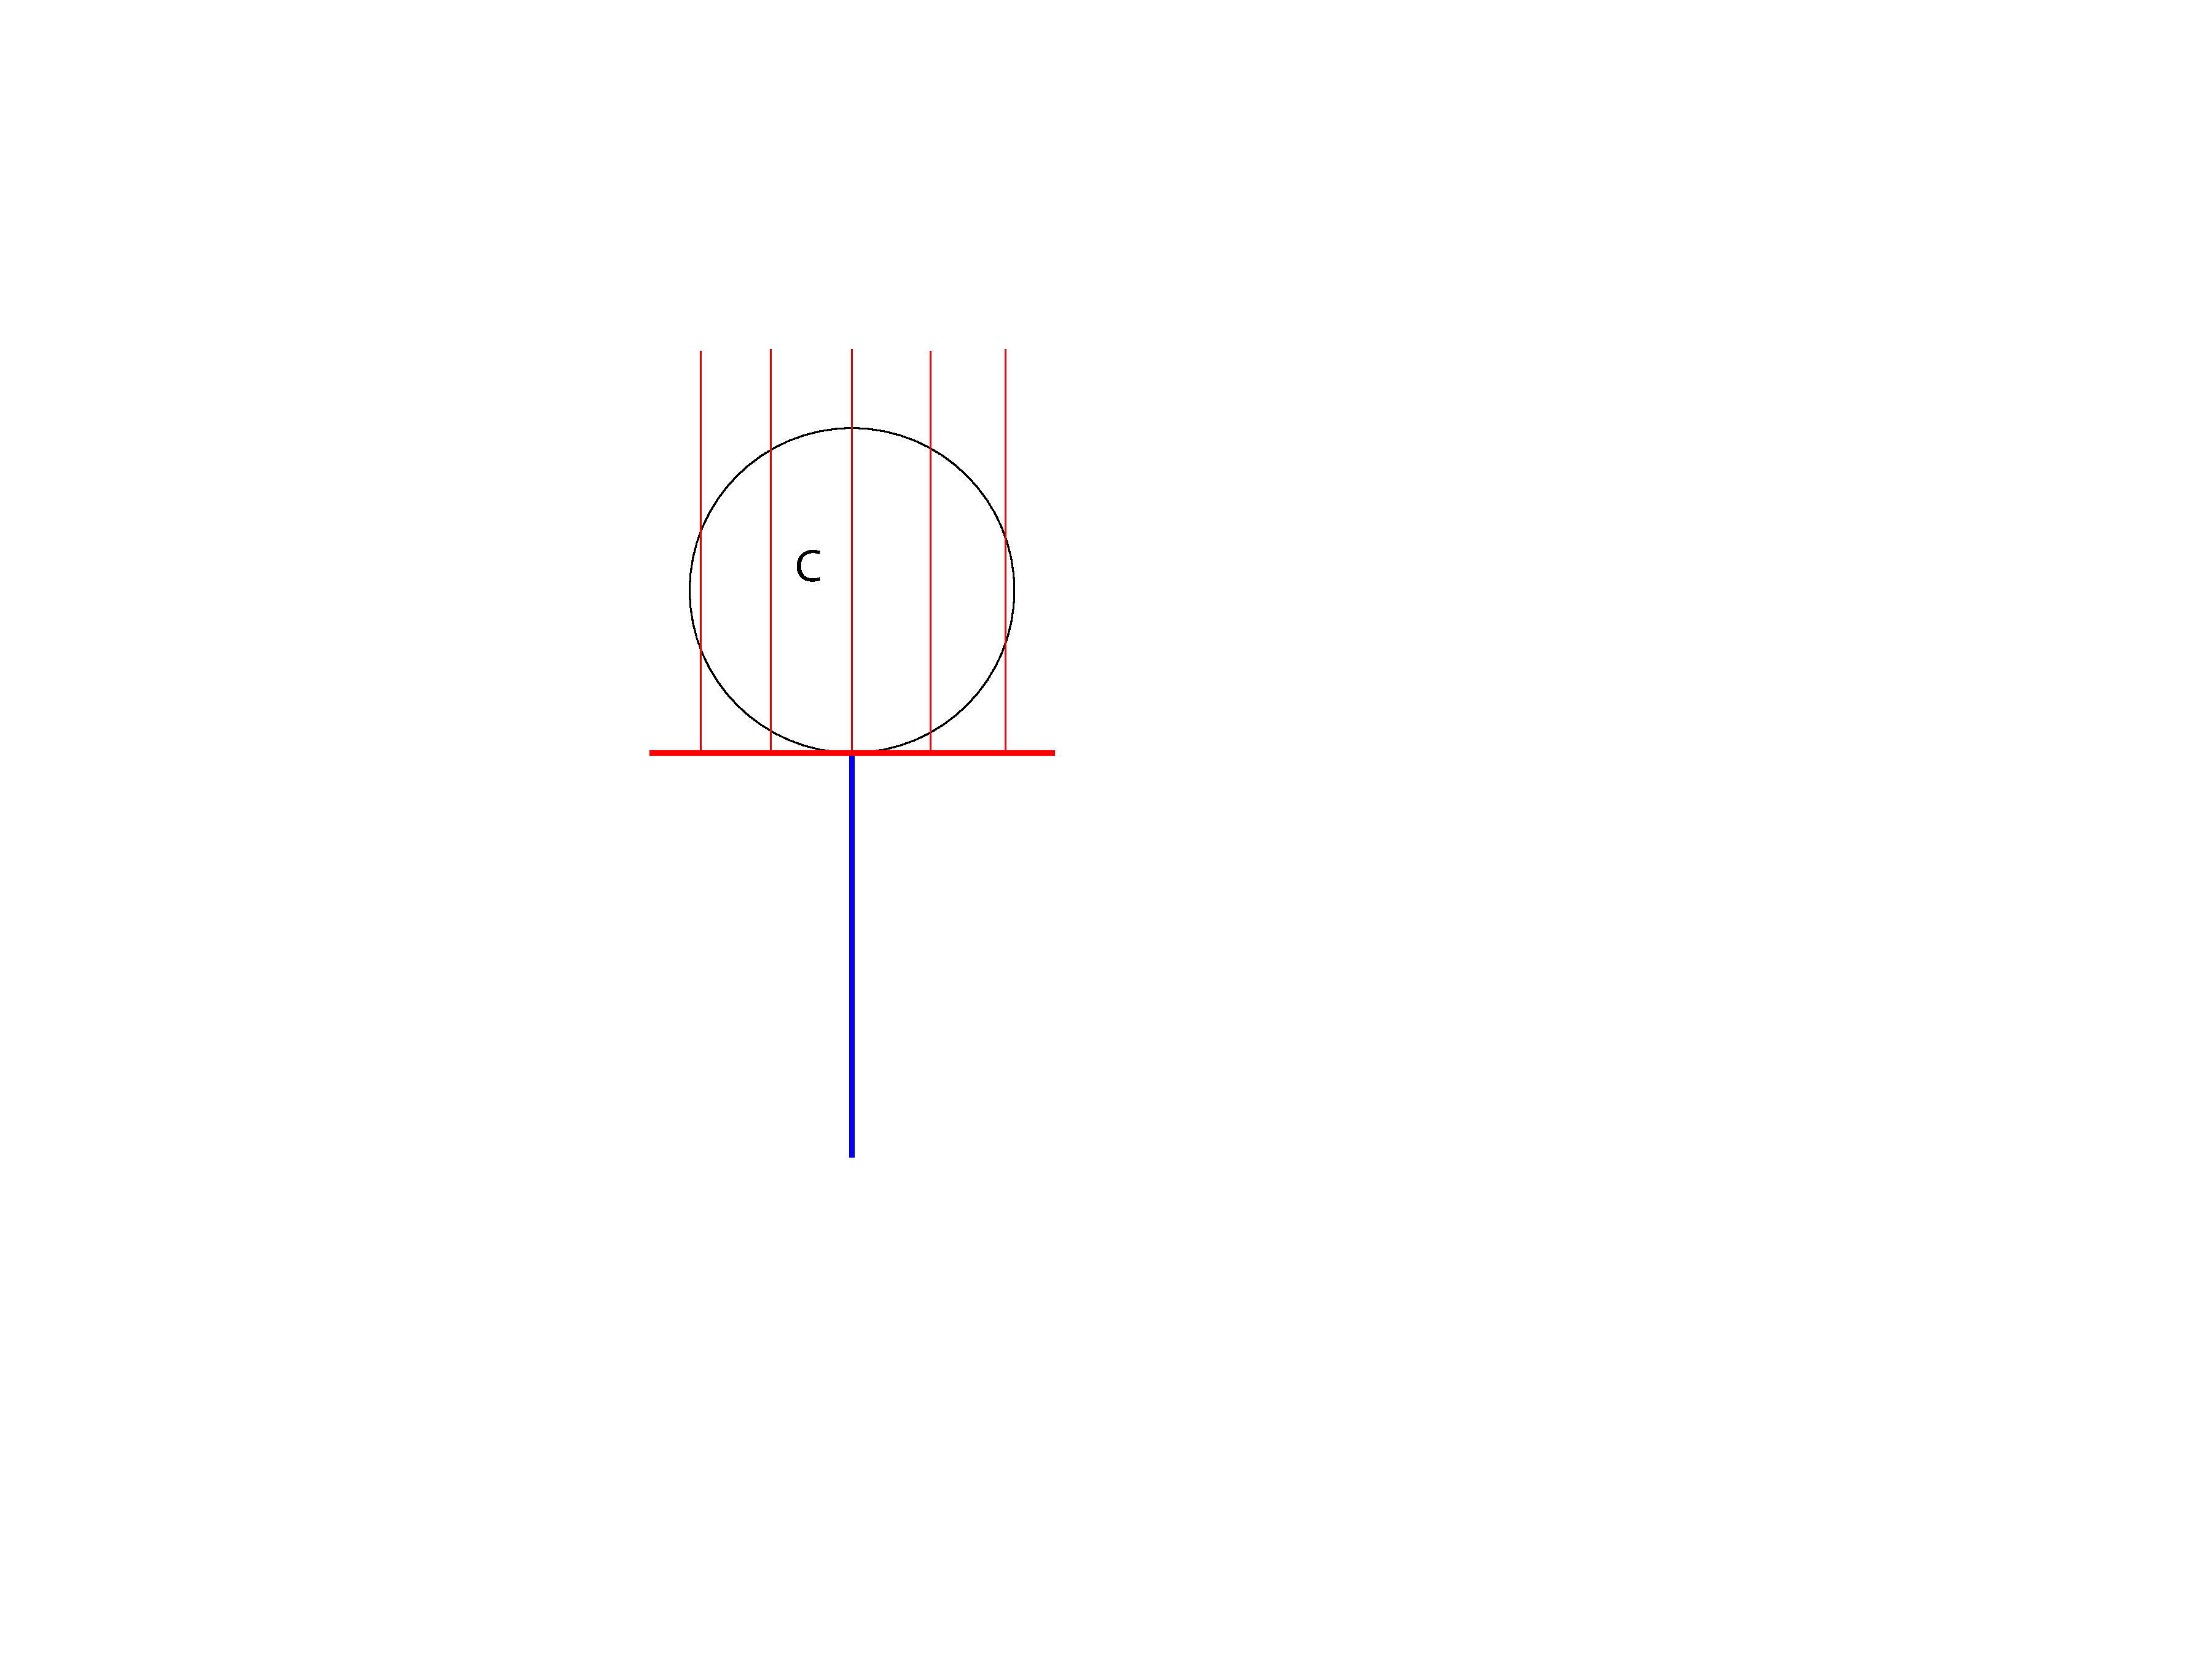
\includegraphics[width=3\textwidth]{figures/lecture13-normal_tangent2.pdf} % second figure itself
        % \caption{second figure}
    \end{minipage}
    \hspace{5cm}
    \vspace{-5cm}
    \caption{Black set is C, red set is $T_C(x)$, blue set is $N_c(x)$}
\end{figure}


% \begin{figure}
% \centering
% \begin{subfigure}{.5\textwidth}
%   \centering
%   \includegraphics[width=8cm]{normal_tangent_cone.pdf}
%   \caption{A subfigure}
%   \label{fig:sub1}
% \end{subfigure}%
% \begin{subfigure}{.5\textwidth}
%   \centering
%   \includegraphics[width=8cm]{normal_tangent2.pdf}
%   \caption{A subfigure}
%   \label{fig:sub2}
% \end{subfigure}
% \caption{A figure with two subfigures}
% \label{fig:test}
% \end{figure}


Suppose we want to minimize a continuously differentiable function $f$ over the intersection of a closed convex set $\Omega$ and an affine set $\mathcal{A} = \{x: Ax=b\}$\begin{equation} \label{eq:constr-opt-affine}
  \begin{array}{ll}
  \text{minimize} &f(x)\\
  \text{subject to} &x \in \Omega\\
  & Ax=b
  \end{array}
  \end{equation}
where $A$ is again a full rank $n\times d$ matrix.  In this section, we will generalize~\eqref{eq:opt-cond} to show

\begin{proposition}\label{prop:constr-opt-affine} $x_\star$ is optimal for~\eqref{eq:constr-opt-affine} if and only if there exists $\lambda_\star \in \R^n$ such that
\[
 \begin{cases}
 - \nabla [f(x_\star) + A^{\trans} \lambda_\star] \in \mathcal{N}_{\Omega} (x_\star)\\
  x_\star \in \Omega \cap \mathcal{A}
  \end{cases}\,.
 \]
\end{proposition}
The key to our analysis here will be to rely on convex analytic arguments. Note that when there is no equality constraint $Ax = b$, our constrained optimality condition is completely equivalent to the assertion
\begin{equation}\label{eq:opt-cond-basic}
  - \nabla f(x_\star) \in \mathcal{N}_{\Omega}(x_\star)\,.
 \end{equation}
Thus, to prove Proposition~\ref{prop:constr-opt-affine}, it will suffice for us to understand the normal cone of the set $\Omega \cap \mathcal{A}$
at the point $x_\star$. To obtain a reasonable characterization, we begin by proving a general fact.
 
\begin{proposition}\label{prop:normal-cone-intersection}
Let $\Omega \subseteq \R^d$ be a closed convex set.  Let $\mathcal{A}$ denote the affine set $\{x~:~Ax = b\}$ for some $A \in \R^{n \times d}$ and $b \in \R^n$.  Suppose that the set $\operatorname{ri}(\Omega) \cap \mathcal{A}$ is non-empty. Then for any $x \in \Omega \cap \mathcal{A}$,
$$\mathcal{N}_{\Omega \cap \mathcal{A}} (x)= \mathcal{N}_{\Omega}(x) + \{A^T \lambda~:~\lambda \in \R^n\}\,.$$
\end{proposition}

\begin{proof}
The ``$\supseteq$'' assertion is straightforward.  To see this, suppose $z \in \Omega \cap \mathcal{A}$ and note that $z-x \in \operatorname{null}(A)$ so that $(z-x)^\trans A^\trans \lambda = \lambda^\trans A(z-x) = 0$ for all $\lambda \in \R^n$. If $u \in \mathcal{N}_{\Omega}(x)$, then $(z-x)^\trans u \le 0$, so for $\lambda\in \R^n$, we have
\[
	\langle z-x, u + A^\trans \lambda \rangle = \langle z-x,u \rangle \leq 0
\]
implying that $u+A^\trans \lambda \in \mathcal{N}_{\Omega \cap \mathcal{A}}(x)$. For the reverse inclusion, let $v \in \mathcal{N}_{\Omega \cap \mathcal{A}}(x)$.  Then we have
\[
	v^\trans (z-x) \leq 0 \text{ for all $z \in \Omega \cap \mathcal{A}$}
\]
Now define the sets
\[
\begin{aligned}
	C_1 &=\left\{ (y,\mu) \in \R^{d+1}~:~ y =z-x,\,\, z\in \Omega,\,\,\mu \leq v^\trans y\right\}\\
	C_2 &= \left\{ (y,\mu) \in \R^{d+1}~:~ y \in \operatorname{ker}(A),\,\,\mu = 0\right\}\,.
\end{aligned}
\]
Note that $\operatorname{ri}(C_1) \cap C_2 = \emptyset$ because otherwise there would exist a $(\hat{y},\hat{\mu})$ such that
\[
	v^\trans \hat{y} > \hat{\mu} = 0
\]
and $\hat{y} \in \mathcal{T}_{\Omega \cap \mathcal{A}}(x)$.  This would contradict our assumption that
$v \in \mathcal{N}_{\Omega \cap \mathcal{A}}(x)$.  Since their intersection is empty, we can properly separate $\operatorname{ri}(C_1)$ from $C_2$.  Indeed, since $C_2$ is a subspace and $C_1$ has nonempty relative interior, there must be a $(w,\gamma)$ such that
\[
	\inf_{(y,\mu)\in C_1} \{ w^\trans y + \gamma \mu\} <	\sup_{(y,\mu)\in C_1} \{ w^\trans y + \gamma \mu\} \leq 0
\]
while
\[
	w^\trans u = 0 \text{ for all $u \in \ker(A)$.}
\]
In particular, this means that $w=A^T \lambda$  for some $\lambda \in \R^n$. Now, $\gamma$ must be nonnegative, as otherwise, 
\[
	\sup_{(y,\mu)\in C_1} \{ w^\trans y + \gamma \mu\} = \infty
\]
(which can be seen by letting $\mu$ tend to negative infinity).  If $\gamma=0$, then
\[
	\sup_{y \in C_1} w^\trans y \leq 0
\]
but the set $\{y~:~w^T y = 0\}$ does not contain the set $\{z-x~:~z\in\Omega\}$ as the infimum is strictly negative.  This means that the relative interior of $\Omega -\{x\}$ cannot intersect the kernel of $A$ which contradicts our assumptions.  Thus, we can conclude that $\gamma$ is strictly positive.  By homogeneity, we may as well assume that $\gamma = 1$.

To complete the argument, note that we now have
\[
 	 (w+v)^\trans (z-x)  \leq 0 \text{ for all $z \in \Omega$.}
\]
This means that $v+w \in \mathcal{N}_{\Omega}(x)$ and we have already shown that $w = A^T\lambda$. Thus, 
\[
v = (v+w)-w \in \mathcal{N}_{\Omega}(x) + \mathcal{N}_{\mathcal{A}}(x)\,.
\]
\end{proof}



Let's now translate the consequence of this proposition for our problem.  Using~\eqref{eq:opt-cond-basic} and Proposition~\ref{prop:normal-cone-intersection}, we have that $x_\star$ is optimal for 
 $$ \min f(x)\;\;\; s.t \;\;\; x \in \Omega, \;\; Ax = b$$ 
 if and only if  $Ax_\star = b$ and there exists a $\lambda \in \R^n$ such that 
 $$ - \nabla [f(x_*) + A^\trans \lambda] \in \mathcal{N}_{\Omega} (x_\star) \;\;\;\; \forall x \in \Omega\,.$$
 This reduction is not immediately useful to us, as it doesn't provide an algorithmic approach to solving the constrained optimization problem.  However, it will form the basis of our dive into duality.
 
 
\subsection{Duality}
 
 Duality lets us associate to any constrained optimization problem, a concave maximization problem whose solutions lower bound the optimal value of the original problem.  In particular, under mild assumptions, we will show that one can solve the primal problem by first solving the dual problem.  
 
We'll continue to focus on the standard primal problem for an equality constrained optimization problem:
  \begin{equation}\label{eq:std-opt}
  \begin{array}{ll}
  \text{minimize} & f(x) \\
  \text{subject to} & x\in\Omega\\
  &Ax = b
    \end{array}
  \end{equation}
 Here, assume that $\Omega$ is a closed convex set, $f$ is differentiable, and $A$ is full rank.
 
 The key behind duality (here, Lagrangian duality) is that problem~\eqref{eq:std-opt} is equivalent to
\[
\min_{x \in \Omega} \max_{\lambda \in \R^n} f(x) + \lambda^T(Ax-b)
\]
To see this, just note that if $Ax\neq b$, then the max with respect to $\lambda$ is infinite.  On the other hand, if $Ax=b$ is feasible, then the max with respect to $\lambda$ is equal to $f(x)$.
 
 The \emph{dual problem} associated with~\eqref{eq:std-opt} is
 \[
 \max_{\lambda \in \R^n} \min_{x \in \Omega} f(x) + \lambda^T(Ax-b)
\]

Note that the function
\[
	q(\lambda): =  \min_{x \in \Omega} f(x) + \lambda^T(Ax-b)
\]
is always a concave function as it is a minimum of linear functions.  Hence the dual problem is a concave maximization problem, regardless of what form $f$ and $\Omega$ take.  We now show that it always lower bounds the primal problem. 

\subsection{Weak duality}
  
\begin{proposition}
For any function $\varphi(x,z)$,
\[
 \min_x \max_z \varphi(x,z) \geq \max_z \min_x \varphi(x,z)\,.
 \]
\end{proposition}
\begin{proof}
The proof is essentially tautological.  Note that we always have
\begin{align*}
\varphi(x,z) &\geq \min_x \varphi(x,z)
\end{align*}
Taking the maximization with respect to the second argument verifies that
\begin{align*}
\max_z \varphi(x,z) &\geq \max_z \min_x \varphi(x,z) \quad \forall x\,.
\end{align*}
Now, minimizing the left hand side with respect to $x$ proves
\begin{align*}
\min_x \max_z\varphi(x,z) &\geq \max_z \min_x \varphi(x,z)
\end{align*}
which is precisely our assertion.
\end{proof}

\subsection{Strong duality}

For convex optimization problems, we can prove a considerably stronger result.  Namely, that the primal and dual problems attain the same optimal value.  And, moreover, that if we know a dual optimal solution, we can extract a primal optimal solution from a simpler optimization problem.

\begin{theorem}[Strong Duality]\quad\\
\begin{enumerate}
\item If $\exists z \in \operatorname{rel int} (\Omega) $ that also satisfies our equality constraint,  and the primal problem has an optimal solution, then the dual has an optimal solution and the primal and dual values are equal
\item In order for $x_\star$ to be optimal for the primal and $\lambda_\star$ optimal for the dual, it is necessary and sufficient that $Ax_\star = b$ , $x_\star \in \Omega$ and $$x_\star \in \arg\min_{x\in \Omega}\;\; \mathcal{L} (x , \lambda_\star) = f(x) + {\lambda_\star}^T (Ax - b)$$
\end{enumerate}
\end{theorem}
\begin{proof}
For all $\lambda$ and all feasible $x$
\begin{align*}
q(\lambda)&\leq  f(x) + \lambda(Ax -b)= f(x)
\end{align*}
where the second equality holds because $Ax=b$.

Now by Proposition~\ref{prop:constr-opt-affine}, $x_\star$ is optimal if and only if there exists a $\lambda_\star$ such that
\[
 \langle \nabla f(x_\star) + A^T \lambda_\star, x- x_\star \rangle \geq 0~~\forall x\in \Omega\\
 \]
and $Ax_\star=b$.  Note that this condition means that $x_\star$ minimizes $\mathcal{L}(x,\lambda_\star)$ over $\Omega$.

  By preceding argument, it now follows that
  \begin{align*} 
  q(\lambda_\star) &= \inf_{x \in \Omega} \mathcal{L}(x, \lambda_\star)\\
  &= \mathcal{L}(x_\star, \lambda_\star)\\
  & = f(x_\star) + {\lambda_\star}^T(Ax_\star - b) = f(x_\star)
  \end{align*}
  which completes the proof.
\end{proof}  
